% Neural Networks

\begin{frame}
  \centering
  \Huge
  \color{orange}
  \vspace{0.2cm}
  Neural Networks
  \vspace{0.5cm}

  \only<2>{
  
\includegraphics[scale=0.35]{nn-meme}
  }
\end{frame}

\begin{slide}{Neural Networks: Biological Motivation}
  \centering
  \pause
  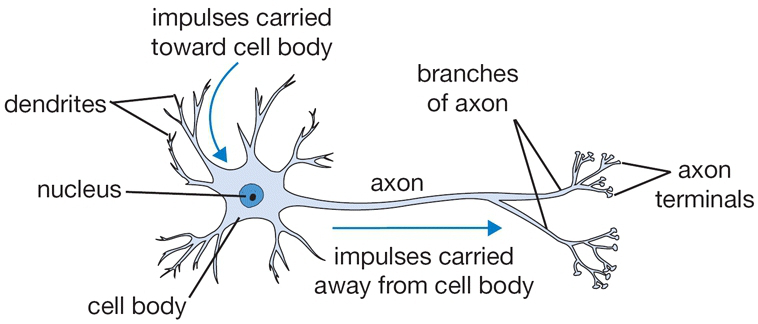
\includegraphics[scale=0.25]{bio-neuron}
  \cite{karpathy1}
  \vspace{0.3cm}
  % 86 Million Neurons
  \begin{itemize}
    \pitem Receive electrochemical signals through \emph{dendrites}
    \pitem Fire their own signal if the input exceeds some threshold
    \pitem Forward their signals via \emph{axons}
    \pitem Connected via \emph{synapses}, which control the strength of interaction % (multiplicative factor)
    \pitem The dynamic alteration of synaptic strengths are the primary source of human \emph{learning} % in this simplified model at least
    % Pavlovian example: human rings bell, dog salivates. So the corresponding connections between the parts of the brain responsible for hearing (the neurons responsible for reacting to this bell noise) and the part responsible for salivation (I'm hungry mode) have strong synaptic connections, so that their stimuli are closely correlated.
  \end{itemize}
\end{slide}

\begin{slide}{Neural Networks: Mathematical Model}
  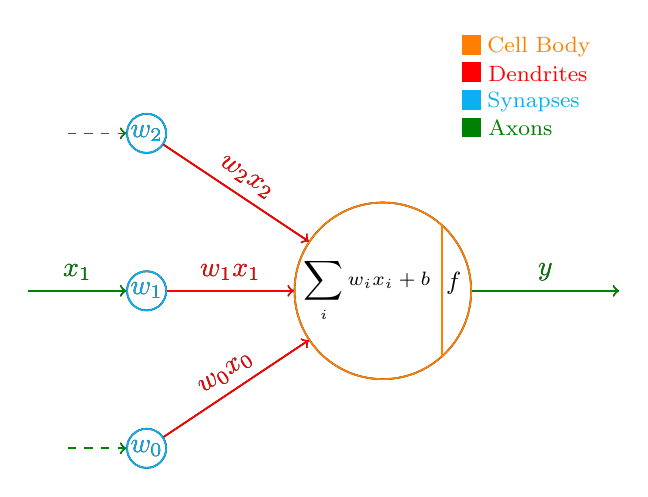
\begin{tikzpicture}[semithick]
    % Cell Body
    \onslide<1> {
      \path (0, 0) coordinate [draw, circle, text width=2cm] (n);
    }
    \onslide<2-> {
      \path [orange] (0, 0) coordinate [draw, circle, text width=2cm] (n);
    }

    % Cell Body Label
    \draw (-0.2, 0) node {\scriptsize$\displaystyle\sum_i w_ix_i + b$};

    % Activation function
    \draw (0.9, 0.1) node {\small$f$};
    \onslide<1>{
    \draw (0.75, 0) -- +(0, 0.84) (0.75, 0) -- +(0, -0.84);
    }
    \onslide<2->{
    \draw [orange] (0.75, 0) -- +(0, 0.84) (0.75, 0) -- +(0, -0.84);
    }

    % Synapses
    \onslide<1-3> {
    \path (-3, -2) coordinate [draw, circle, inner sep=5pt]
          (s0) node {$w_0$};
    }
    \onslide<4-> {
    \path [ProcessBlue] (-3, -2) coordinate [draw, circle, inner sep=5pt]
          (s0) node {$w_0$};
    }

    \onslide<1-3> {
    \path (-3, 0) coordinate [draw, circle, inner sep=5pt]
          (s1) node {$w_1$};
    }
    \onslide<4-> {
    \path [ProcessBlue] (-3, 0) coordinate [draw, circle, inner sep=5pt]
          (s1) node {$w_1$};
    }

    \onslide<1-3> {
    \path (-3, 2) coordinate [draw, circle, inner sep=5pt]
          (s2) node {$w_2$};
    }
    \onslide<4-> {
    \path [ProcessBlue] (-3, 2) coordinate [draw, circle, inner sep=5pt]
          (s2) node {$w_2$};
    }

    % Dendrites
    \onslide<-2> {
    \draw [->] (s0) -- (n) node [midway, above, sloped] {$w_0x_0$};
    }
    \onslide<3-> {
    \draw [Red, ->] (s0) -- (n) node [midway, above, sloped] {$w_0x_0$};
    }

    \onslide<-2> {
    \draw [->] (s1) -- (n) node [midway, above, sloped] {$w_1x_1$};
    }
    \onslide<3-> {
    \draw [Red, ->] (s1) -- (n) node [midway, above, sloped] {$w_1x_1$};
    }

    \onslide<-2> {
    \draw [->] (s2) -- (n) node [midway, above, sloped] {$w_2x_2$};
    }
    \onslide<3-> {
    \draw [Red, ->] (s2) -- (n) node [midway, above, sloped] {$w_2x_2$};
    }

    % Input Axon from other Neuron
    \onslide<-4>{
    \draw [->] (-4.5, 0) -- (s1) node [midway, above] {$x_1$};
    }
    \onslide<5->{
    \draw [Green, ->] (-4.5, 0) -- (s1) node [midway, above] {$x_1$};
    }

    \onslide<-4>{
    \draw [dashed, ->] (-4, -2) -- (s0);
    }
    \onslide<5->{
    \draw [Green, dashed, ->] (-4, -2) -- (s0);
    }

    \onslide<-4>{
    \draw [dashed, ->] (-4, 2) -- (s2);
    }
    \onslide<5->{
    \draw [Green, dashed, ->] (-4, 2) -- (s2);
    }

    % Output Axon
    \onslide<-4>{
    \draw [->] (n) -- ++(3, 0) node [midway, above] {$y$};
    }
    \onslide<5->{
    \draw [Green, ->] (n) -- ++(3, 0) node [midway, above] {$y$};
    }

    % Legend
    \onslide<2->{
    \fill [orange] (1, 3) rectangle ++(0.25, 0.25)
          node [pos=0.4, right] {\hspace{0.1cm}\footnotesize Cell Body};
    }

    \onslide<3->{
    \fill [Red] (1, 2.65) rectangle ++(0.25, 0.25)
          node [pos=0.45, right] {\hspace{0.1cm}\footnotesize Dendrites};
    }

    \onslide<4->{
    \fill [ProcessBlue] (1, 2.3) rectangle ++(0.25, 0.25)
          node [pos=0.4, right] {\hspace{0.1cm}\footnotesize Synapses};
    }

    \onslide<5->{
    \fill [Green] (1, 1.95) rectangle ++(0.25, 0.25)
          node [pos=0.45, right] {\hspace{0.1cm}\footnotesize Axons};
    }
  \end{tikzpicture}
\end{slide}

\begin{slide}{Artificial Neural Networks}
  \begin{itemize}
    \item<2-> First attempt at Artificial Neural Network (ANN) by McCulloch and Pitts in 1943
    \item<3-> Summed binary inputs and thresholded them
    \item<4-> Could learn AND, NOT and OR functions
  \end{itemize}
  \vspace{1cm}

  \onslide<3->{
  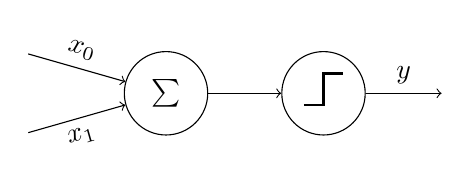
\begin{tikzpicture}
    % Sum
    \path (0, 0) coordinate [draw, circle, text width=0.8cm] (n) node {$\sum$};

    % Inputs
    \draw [->] (-1.75, 0.5) -- (n) node [midway, above, sloped] {$x_0$};
    \draw [->] (-1.75, -0.5) -- (n) node [midway, below, sloped] {$x_1$};

    % Threshold unit
    \path (2, 0) coordinate [draw, circle, text width=0.8cm] (t);
    \draw [thick] (1.75, -0.15) -- ++(0.25, 0) -- ++(0, 0.4) -- ++(0.25, 0);

    % Output
    \draw [->] (n) -- (t);
    \draw [->] (t) -- ++(1.5, 0) node [midway, above] {$y$};
  \end{tikzpicture}
  }
\end{slide}

\begin{slide}{Artificial Neural Networks}
  \begin{itemize}
    \item<1-> Frank Rosenblatt improved on this model in 1957
    \item<2-> He \emph{weighted} the inputs and added a bias
    % The bias means we can not only learn all linear but all affine functions
    \item<3-> This models the synaptic strengths between axons and dendrites
    \item<4-> He called this model a \emph{Perceptron}
  \end{itemize}
  \vspace{0.5cm}

  \onslide<2->{
  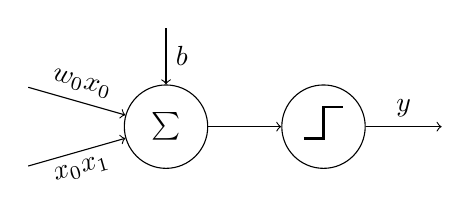
\begin{tikzpicture}
    % Sum
    \path (0, 0) coordinate [draw, circle, text width=0.8cm] (n) node {$\sum$};

    % Inputs
    \draw [->] (-1.75, 0.5) -- (n) node [midway, above, sloped] {$w_0x_0$};
    \draw [->] (-1.75, -0.5) -- (n) node [midway, below, sloped] {$x_0x_1$};

    % Bias
    \draw [->] (0, 1.25) -- (n) node [midway, right] {$b$};

    % Threshold unit
    \path (2, 0) coordinate [draw, circle, text width=0.8cm] (t);
    \draw [thick] (1.75, -0.15) -- ++(0.25, 0) -- ++(0, 0.4) -- ++(0.25, 0);

    % Output
    \draw [->] (n) -- (t);
    \draw [->] (t) -- ++(1.5, 0) node [midway, above] {$y$};
  \end{tikzpicture}
  }
\end{slide}

\renewcommand{\thealgorithm}{}
\begin{slide}{Artificial Neural Networks}
  \begin{itemize}
    \pitem Because the Perceptron has parameters, it can be trained
    \pitem First supervised learning algorithm for ANNs:
  \end{itemize}
  \pause
  \begin{algorithm}[H]
  \caption{Train Perceptron}
  \begin{algorithmic}
  \State Input: A dataset of $(\mathbf{x}, \hat{y})$ pairs
  \State Output: Trained Perceptron
  \ForAll{$(\mathbf{x}, \hat{y})$ in dataset}:
    \State $y \gets f(\mathbf{w}^\top \mathbf{x} + b)$
    \If {$y \neq \hat{y}$}
      \If {$\hat{y} = 0 \land y = 1$}
        \State Decrease all weights $w_i$ where $x_i$ was $1$
      \ElsIf {$\hat{y} = 1 \land y = 0$}
        \State Increase all weights $w_i$ where $x_i$ was $1$
      \EndIf
    \EndIf
  \EndFor
  \end{algorithmic}
  \end{algorithm}
\end{slide}

\begin{slide}{Artificial Neural Networks}
  \begin{itemize}
    \item<1-> Perceptrons even work for multi-class classification
    \item<2-> Just use more perceptrons
    \item<5-> This is now a \emph{multilayer perceptron} (MLP)
  \end{itemize}
  \vspace{0.3cm}

  \onslide<2->{
  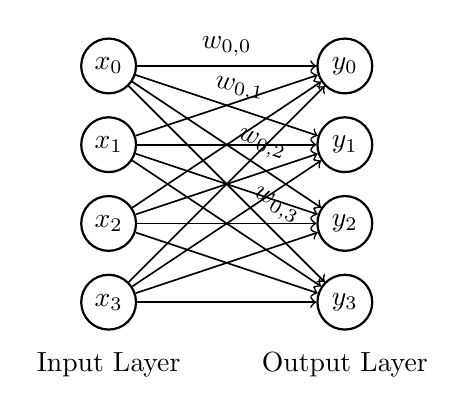
\begin{tikzpicture}
    % Input layer
    \foreach \i in {0, ..., 3} {
      \path (0, {-\i}) coordinate [draw, circle, thick, inner sep=7pt]
            (x\i) node {$x_\i$};
    }
    \draw (0, -3.8) node {Input Layer};

    % Output layer
    \foreach \i in {0, ..., 3} {
      \path (3, {-\i}) coordinate [draw, circle, thick, inner sep=7pt]
            (y\i) node {$y_\i$};
    }
    \draw (3, -3.8) node {Output Layer};

    % Connections
    \onslide<3->{
      \foreach \i in {0, ..., 3} {
        \foreach \j in {0, ..., 3} {
          \ifnum\i=0
            \draw [semithick, ->] (x\i) -- (y\j);
          \else
            \onslide<5-> {
              \draw [semithick, ->] (x\i) -- (y\j);
            }
          \fi
        }
        \ifnum\i=0
          \onslide<4>{
            \draw [line width=0] (x0) -- (y0)
                  node [above, midway] {$w_{0,0}$};

            \draw [line width=0] (x0) -- (y1)
                  node [above, pos=0.55, rotate=-10] {$w_{0,1}$};

            \draw [line width=0] (x0) -- (y2)
                  node [above, pos=0.65, rotate=-20] {$w_{0,2}$};

            \draw [line width=0] (x0) -- (y3)
                  node [above, pos=0.7, rotate=-30] {$w_{0,3}$};
          }
        \fi
      }
    }
  \end{tikzpicture}
  }
\end{slide}

\begin{slide}{Artificial Neural Networks}
  \frameheader{NEW NAVY DEVICE LEARNS BY DOING}
  \begin{quote}
    WASHINGTON, July 7 (UPI) -- The Navy revealed the embryo of an electronic computer today that it expects will be able to walk, talk, see, write, reproduce itself and be conscious of its existence.
  \end{quote}

\begin{flushleft}
  \cite{nyt}
\end{flushleft}
\end{slide}

\begin{frame}
  \centering
  
\includegraphics[scale=0.4, trim={0 4.5cm 0 0}, clip]{woman-50s}
\end{frame}

\begin{slide}{Artificial Neural Networks}
  \begin{itemize}
    \item<1-> Perceptrons have one fundamental problem
    \item<2-> They can only learn linear functions
  \end{itemize}

  \onslide<3->{
  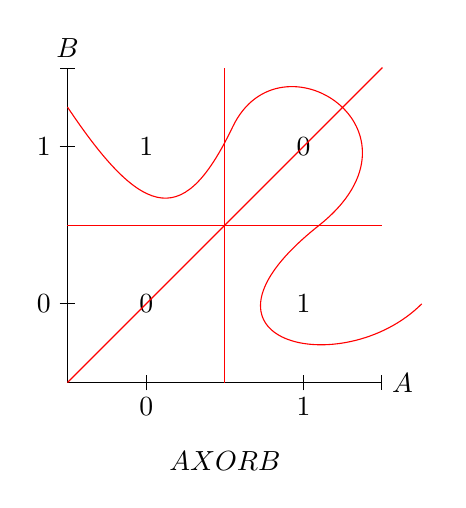
\begin{tikzpicture}
    % A axis
    \draw [-|] (0, 0) -- ++(4, 0) node [right] {$A$};

    % B axis
    \draw [-|] (0, 0) -- ++(0, 4) node [above] {$B$};

    % Ticks
    \foreach \i in {0, 1} {
      % A Axis
      \draw ({\i*2+1)}, -0.1) -- ++(0, 0.2);
      \draw ({\i*2+1)}, -0.3) node {$\i$};

      % B Axis
      \draw (-0.1, {\i*2+1)}) -- ++(0.2, 0);
      \draw (-0.3, {\i*2+1)}) node {$\i$};
    }

    % XOR values
    \draw (1, 1) node {$0$};
    \draw (3, 1) node {$1$};
    \draw (3, 3) node {$0$};
    \draw (1, 3) node {$1$};

    % Caption
    \draw (2, -1) node {$A \text{ XOR } B$};

    \onslide<4>{\draw [red] (0, 0) -- (4, 4);}
    \onslide<5>{\draw [red] (2, 0) -- (2, 4);}
    \onslide<6>{\draw [red] (0, 2) -- (4, 2);}
    \onslide<7>{
      \draw [red] (0, 3.5)
            .. controls (1, 2) and (1.5, 2)
            .. (2.1, 3.25)
            .. controls (2.7, 4.5) and (4.7, 3.2)
            .. (3.2, 2)
            .. controls (1.3, 0.5) and (3.5, 0)
            .. (4.5, 1);
    }
  \end{tikzpicture}
  }
\end{slide}

\begin{slide}{Artificial Neural Networks}
  \begin{itemize}
    \item<1-> The solution:
    \begin{itemize}
      \item<2-> A hidden layer
      \item<3-> With \emph{non-linear} activation functions
    \end{itemize}
  \end{itemize}
  \vspace{0.75cm}

  \onslide<4->{
  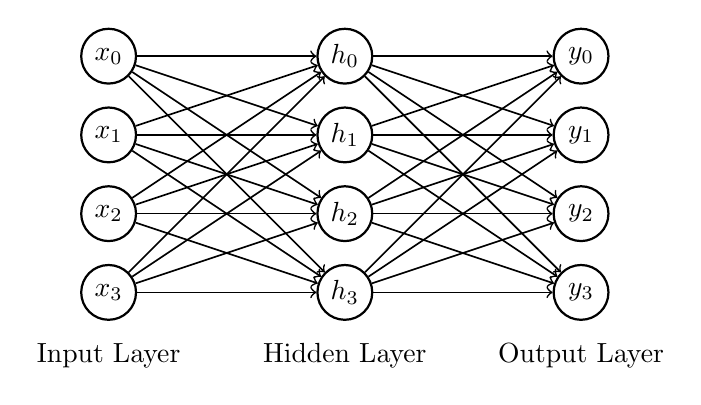
\begin{tikzpicture}
    % Input layer
    \foreach \i in {0, ..., 3} {
      \path (0, {-\i}) coordinate [draw, circle, thick, inner sep=7pt]
            (x\i) node {$x_\i$};
    }
    \draw (0, -3.8) node {Input Layer};

    % Output layer
    \foreach \i in {0, ..., 3} {
      \path (3, {-\i}) coordinate [draw, circle, thick, inner sep=7pt]
            (h\i) node {$h_\i$};
    }
    \draw (3, -3.8) node {Hidden Layer};

    % Output layer
    \foreach \i in {0, ..., 3} {
      \path (6, {-\i}) coordinate [draw, circle, thick, inner sep=7pt]
            (y\i) node {$y_\i$};
    }
    \draw (6, -3.8) node {Output Layer};

    % Connections
      \foreach \i in {0, ..., 3} {
        \foreach \j in {0, ..., 3} {
            \draw [semithick, ->] (x\i) -- (h\j);
            \draw [semithick, ->] (h\i) -- (y\j);
        }
      }
  \end{tikzpicture}
  }
\end{slide}

\begin{slide}{Activation Functions}
  \begin{itemize}
    \item Three important activation functions
  \end{itemize}
  \only<1>{\vspace{5.8cm}}
  \vspace{0.5cm}
  \only<2>{
  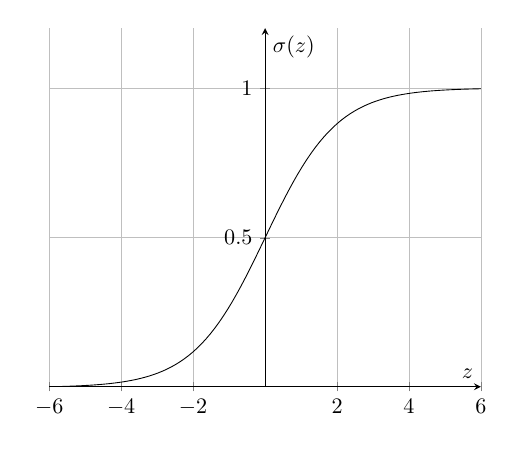
\begin{tikzpicture}[scale=0.8]
    \begin{axis}[
        xlabel=$z$,
        ylabel=$\sigma(z)$,
        ytick={0.5, 1},
        ymax=1.2,
        axis lines=center,
        grid,
        y label style={at={(ticklabel* cs:1)}}
      ]
      \addplot [domain=-6:6, samples=100] {1/(1 + exp(-\x))};
    \end{axis}
  \end{tikzpicture}

  Le \emph{Sigmoid}
  % Undesirable properties:
  % 1. Not zero centered (always outputs positive values), which can have bad implications for GD
  % 2. Function saturates for very large or very small values of x, i.e. the gradient will be zero for large inputs. This means that during backprop, which computes the chain rule and thus multiplies this gradient with other gradients, will become zero and the network will no longer learn. Also it's data (i.e. the units before it) will not learn, because this small or zero multiplicative term will be in the chain rule too.
  % Large weights from random initialization can already break this
  % Note about Cousera
  } \only<3>{
  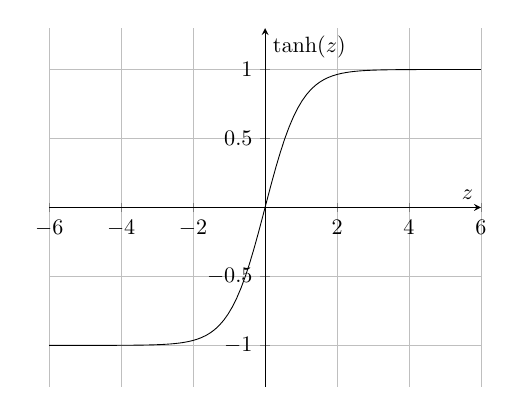
\begin{tikzpicture}[scale=0.8]
    \begin{axis}[
        xlabel=$z$,
        ylabel=$\tanh(z)$,
        ymin=-1.3, ymax=1.3,
        axis lines=center,
        grid,
        y label style={at={(ticklabel* cs:1)}}
      ]
      \addplot [domain=-6:6, samples=100] {tanh(\x))};
    \end{axis}
  \end{tikzpicture}

  El $\tanh$
  % The Tanh is actually 2sigma(2x) - 1
  % Preferred over the sigmoid because it is zero centered
  % Gradient still saturates
  } \only<4> {
  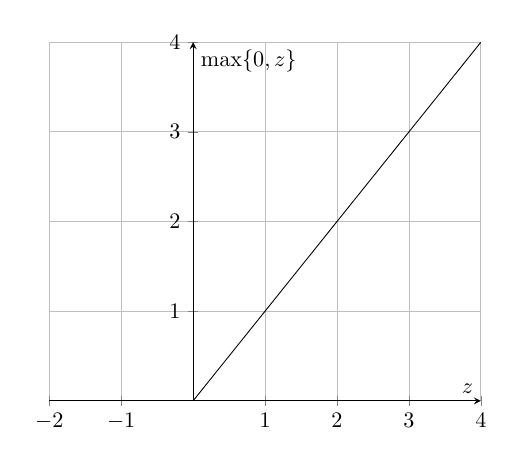
\begin{tikzpicture}[scale=0.8]
    \begin{axis}[
        xlabel=$z$,
        ylabel={$\max\{0, z\}$},
        axis lines=center,
        grid,
        y label style={at={(ticklabel* cs:1)}}
      ]
      \addplot [domain=-2:4] {max(0, \x)};
    \end{axis}
  \end{tikzpicture}

  Das ReLu
  % The most ridiculous linear function you could think of
  % Surpisingly very nice properties
  % Gradient does not saturate for positive values
  % Gradient is very simple, 1 for x > 0 and 0 for x < 0
  % Non-differentiable at x = 0, but x usually never becomes zero because of the bias
  % Have the problem that they can die, when it happens that all data is on the negative side
  % The hope is, e.g. during SGD, that at least one input will be on the steep side
  % Then the Relu still learns
  % But it could happen for example that in one big gradient update the bias becomes very negative
  % Then the relu will always output zero and its gradient is zero
  % So learning stops, no gradient will flow through this neuron any more
  % The leaky relu solves this
}
\end{slide}

\begin{slide}{Neural Networks by Foot}
    \begin{itemize}
      \item<2-> We want to classify programmers into one of two classes
      \begin{enumerate}
        \item<3-> \texttt{l33t h4x0r}
        \item<4-> \texttt{n00b}
      \end{enumerate}
      \item<5-> Two input features:
      \begin{enumerate}
        \item<6-> Maximum number of successive pointers to pointers maintained
        \item<7-> Liters of coffee per year
      \end{enumerate}
      \item<9-> Our labels are \emph{one-hot} encoded
    \end{itemize}
  \only<-7>{\vspace{2.7cm}}
  \only<8>{
  $$
  \mathbf{D} =
  \begin{blockarray}{cc}
    p & c \\
  \begin{block}{[cc]}
    10  & 365\\ % linus torvalds
    3  & 120\\ % me
    0  & 1000\\ % coffee addicted ruby programmer
  \end{block}
  \end{blockarray}
  \hspace{0.5cm}
  $$
  }
  \only<9>{
  $$
  \mathbf{D} =
  \begin{blockarray}{cc}
    p & c \\
  \begin{block}{[cc]}
    10  & 365\\ % linus torvalds
    3  & 120\\ % me
    0  & 1000\\ % coffee addicted ruby programmer
  \end{block}
\end{blockarray}
\hspace{0.5cm}
\mathbf{\hat{Y}} =
  \begin{blockarray}{cc}
    \mathtt{l33t} & \mathtt{n00b} \\
  \begin{block}{[cc]}
    1  & 0\\ % linus torvalds
    1  & 0\\ % me
    0  & 1\\ % coffee addicted ruby programmer
  \end{block}
  \end{blockarray}
  $$
  }
  \only<10>{
  \scalebox{0.7}{
  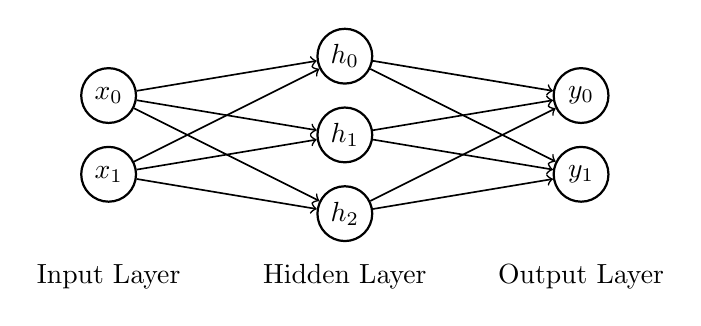
\begin{tikzpicture}
    % Input layer
    \foreach \i in {0, 1} {
      \path (0, {-\i-0.5}) coordinate [draw, circle, thick, inner sep=7pt]
            (x\i) node {$x_\i$};
    }
    \draw (0, -2.8) node {Input Layer};

    % Output layer
    \foreach \i in {0, ..., 2} {
      \path (3, {-\i}) coordinate [draw, circle, thick, inner sep=7pt]
            (h\i) node {$h_\i$};
    }
    \draw (3, -2.8) node {Hidden Layer};

    % Output layer
    \foreach \i in {0, ..., 1} {
      \path (6, {-\i-0.5}) coordinate [draw, circle, thick, inner sep=7pt]
            (y\i) node {$y_\i$};
    }
    \draw (6, -2.8) node {Output Layer};

    % Connections
      \foreach \i in {0, ..., 1} {
        \foreach \j in {0, ..., 2} {
            \draw [semithick, ->] (x\i) -- (h\j);
        }
      }
      \foreach \i in {0, ..., 2} {
        \foreach \j in {0, ..., 1} {
            \draw [semithick, ->] (h\i) -- (y\j);
        }
      }
  \end{tikzpicture}
  }}
\end{slide}

\begin{slide}{Neural Networks by Foot}
  \scalebox{0.7}{
  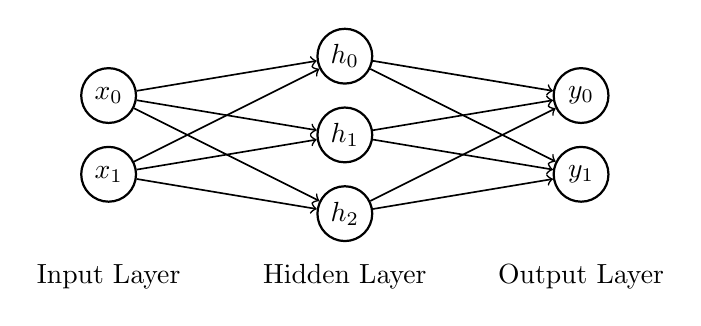
\begin{tikzpicture}
    % Input layer
    \foreach \i in {0, 1} {
      \path (0, {-\i-0.5}) coordinate [draw, circle, thick, inner sep=7pt]
            (x\i) node {$x_\i$};
    }
    \draw (0, -2.8) node {Input Layer};

    % Output layer
    \foreach \i in {0, ..., 2} {
      \path (3, {-\i}) coordinate [draw, circle, thick, inner sep=7pt]
            (h\i) node {$h_\i$};
    }
    \draw (3, -2.8) node {Hidden Layer};

    % Output layer
    \foreach \i in {0, ..., 1} {
      \path (6, {-\i-0.5}) coordinate [draw, circle, thick, inner sep=7pt]
            (y\i) node {$y_\i$};
    }
    \draw (6, -2.8) node {Output Layer};

    % Connections
      \foreach \i in {0, ..., 1} {
        \foreach \j in {0, ..., 2} {
            \draw [semithick, ->] (x\i) -- (h\j);
        }
      }
      \foreach \i in {0, ..., 2} {
        \foreach \j in {0, ..., 1} {
            \draw [semithick, ->] (h\i) -- (y\j);
        }
      }
  \end{tikzpicture}
  }
  $$
  \begin{sbmatrix}{\mathbf{D}}
    10 & 365 \\
    3 & 120 \\
    0 & 1000 \\
  \end{sbmatrix}
  \pause
  \times
  \begin{sbmatrix}{\mathbf{W_1}}
  -0.04 & -0.43 & 0.57 \\
  0.04 & 0.52 & -0.6 \\
  \end{sbmatrix}
  \pause
  \,+_b\,
  \begin{sbmatrix}{\mathbf{b_1}}
    -2.03 & -0.26 & 2.16
  \end{sbmatrix}
  $$
  $$
  \pause
  =
  \begin{sbmatrix}{\mathbf{H}}
  13.37 & 183.66 & -210.46 \\
  3.05 & 60.33 & -67.91 \\
  41.13 & 515.49 & -596.08 \\
  \end{sbmatrix}
  $$
\end{slide}

\begin{slide}{Neural Networks by Foot}
  \scalebox{0.7}{
  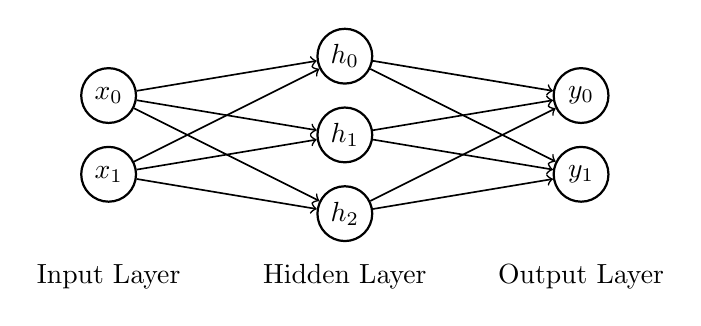
\begin{tikzpicture}
    % Input layer
    \foreach \i in {0, 1} {
      \path (0, {-\i-0.5}) coordinate [draw, circle, thick, inner sep=7pt]
            (x\i) node {$x_\i$};
    }
    \draw (0, -2.8) node {Input Layer};

    % Output layer
    \foreach \i in {0, ..., 2} {
      \path (3, {-\i}) coordinate [draw, circle, thick, inner sep=7pt]
            (h\i) node {$h_\i$};
    }
    \draw (3, -2.8) node {Hidden Layer};

    % Output layer
    \foreach \i in {0, ..., 1} {
      \path (6, {-\i-0.5}) coordinate [draw, circle, thick, inner sep=7pt]
            (y\i) node {$y_\i$};
    }
    \draw (6, -2.8) node {Output Layer};

    % Connections
      \foreach \i in {0, ..., 1} {
        \foreach \j in {0, ..., 2} {
            \draw [semithick, ->] (x\i) -- (h\j);
        }
      }
      \foreach \i in {0, ..., 2} {
        \foreach \j in {0, ..., 1} {
            \draw [semithick, ->] (h\i) -- (y\j);
        }
      }
  \end{tikzpicture}
  }
  $$
  \relu(\mathbf{H})
  \pause
  =
  \max\{0, \mathbf{H}\}
  \pause
  =
  \begin{sbmatrix}{\mathbf{H'}}
    13.37 & 183.66 & 0.0 \\
    3.05 & 60.33 & 0.0 \\
    41.13 & 515.49 & 0.0 \\
  \end{sbmatrix}
  $$
\end{slide}

\begin{slide}{Neural Networks by Foot}
  \scalebox{0.7}{
  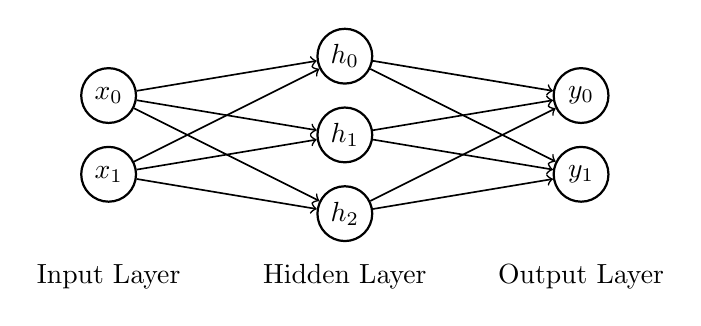
\begin{tikzpicture}
    % Input layer
    \foreach \i in {0, 1} {
      \path (0, {-\i-0.5}) coordinate [draw, circle, thick, inner sep=7pt]
            (x\i) node {$x_\i$};
    }
    \draw (0, -2.8) node {Input Layer};

    % Output layer
    \foreach \i in {0, ..., 2} {
      \path (3, {-\i}) coordinate [draw, circle, thick, inner sep=7pt]
            (h\i) node {$h_\i$};
    }
    \draw (3, -2.8) node {Hidden Layer};

    % Output layer
    \foreach \i in {0, ..., 1} {
      \path (6, {-\i-0.5}) coordinate [draw, circle, thick, inner sep=7pt]
            (y\i) node {$y_\i$};
    }
    \draw (6, -2.8) node {Output Layer};

    % Connections
      \foreach \i in {0, ..., 1} {
        \foreach \j in {0, ..., 2} {
            \draw [semithick, ->] (x\i) -- (h\j);
        }
      }
      \foreach \i in {0, ..., 2} {
        \foreach \j in {0, ..., 1} {
            \draw [semithick, ->] (h\i) -- (y\j);
        }
      }
  \end{tikzpicture}
  }
  $$
  \mathbf{H'}
  \pause
  \times
  \begin{sbmatrix}{\mathbf{W_2}}
    0.44 & 0.19 \\
    -0.04 & 1.14 \\
    0.68 & 0.85 \\
  \end{sbmatrix}
  \pause
  \,+_b\,
  \begin{sbmatrix}{\mathbf{b_2}}
    -0.19 & -0.49 \\
  \end{sbmatrix}
  $$
  \pause
  $$
  =
  \begin{sbmatrix}{\mathbf{Y}}
    -2.53 & 211.85 \\
    -1.55 & 69.01 \\
    -5.16 & 596.17 \\
  \end{sbmatrix}
  $$
\end{slide}

\begin{slide}{Neural Networks by Foot}
  \scalebox{0.7}{
  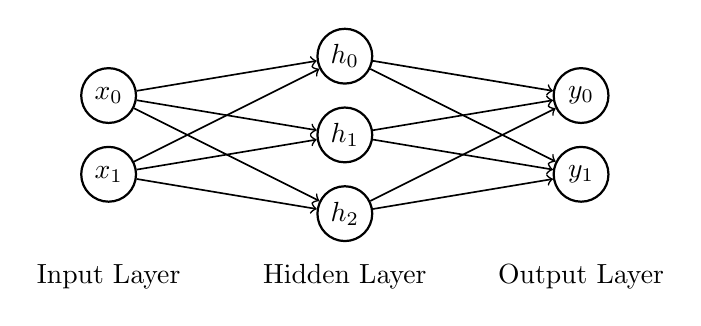
\begin{tikzpicture}
    % Input layer
    \foreach \i in {0, 1} {
      \path (0, {-\i-0.5}) coordinate [draw, circle, thick, inner sep=7pt]
            (x\i) node {$x_\i$};
    }
    \draw (0, -2.8) node {Input Layer};

    % Output layer
    \foreach \i in {0, ..., 2} {
      \path (3, {-\i}) coordinate [draw, circle, thick, inner sep=7pt]
            (h\i) node {$h_\i$};
    }
    \draw (3, -2.8) node {Hidden Layer};

    % Output layer
    \foreach \i in {0, ..., 1} {
      \path (6, {-\i-0.5}) coordinate [draw, circle, thick, inner sep=7pt]
            (y\i) node {$y_\i$};
    }
    \draw (6, -2.8) node {Output Layer};

    % Connections
      \foreach \i in {0, ..., 1} {
        \foreach \j in {0, ..., 2} {
            \draw [semithick, ->] (x\i) -- (h\j);
        }
      }
      \foreach \i in {0, ..., 2} {
        \foreach \j in {0, ..., 1} {
            \draw [semithick, ->] (h\i) -- (y\j);
        }
      }
  \end{tikzpicture}
  }
  $$
    \softmax(\mathbf{Y}) =
    \pause
    \begin{sbmatrix}{\mathbf{Y}}
      0.0 & 1.0 \\
      0.0 & 1.0 \\
      0.0 & 1.0 \\
    \end{sbmatrix}
  $$
\end{slide}

\begin{slide}{Neural Networks By Foot}
  \scalebox{0.7}{
  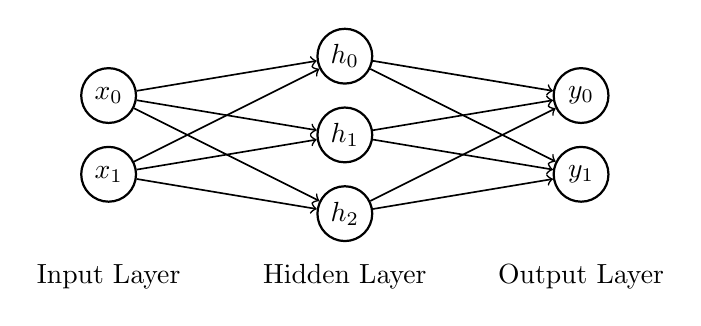
\begin{tikzpicture}
    % Input layer
    \foreach \i in {0, 1} {
      \path (0, {-\i-0.5}) coordinate [draw, circle, thick, inner sep=7pt]
            (x\i) node {$x_\i$};
    }
    \draw (0, -2.8) node {Input Layer};

    % Output layer
    \foreach \i in {0, ..., 2} {
      \path (3, {-\i}) coordinate [draw, circle, thick, inner sep=7pt]
            (h\i) node {$h_\i$};
    }
    \draw (3, -2.8) node {Hidden Layer};

    % Output layer
    \foreach \i in {0, ..., 1} {
      \path (6, {-\i-0.5}) coordinate [draw, circle, thick, inner sep=7pt]
            (y\i) node {$y_\i$};
    }
    \draw (6, -2.8) node {Output Layer};

    % Connections
      \foreach \i in {0, ..., 1} {
        \foreach \j in {0, ..., 2} {
            \draw [semithick, ->] (x\i) -- (h\j);
        }
      }
      \foreach \i in {0, ..., 2} {
        \foreach \j in {0, ..., 1} {
            \draw [semithick, ->] (h\i) -- (y\j);
        }
      }
  \end{tikzpicture}
  }
  \begin{itemize}
    \item<1-> Let $\mathcal{W}$ be $[\mathbf{W}_1, \mathbf{W}_2]$
    \item<2-> Then $J(\mathcal{W})$ is the network's loss
    \item<3-> $\nabla J(\mathcal{W})$ are the gradients
    \item<4-> The final step of this iteration would thus be: $$\mathcal{W} \gets \mathcal{W} - \nabla J(\mathcal{W})$$
  \end{itemize}
\end{slide}

\begin{slide}{Dropout}
  \begin{itemize}
    \item<1-> One recent regularization technique is \emph{Dropout}
    \item<2-> It is used especially for deep neural networks
    \item<3-> Basic idea:
    \begin{itemize}
      \item<4-> We deactivate neurons on each activation with probability $p$
      \item<5-> Can be seen as sampling a new neural network each time
      \item<5-> This prevents neurons from depending too much on each other % A unit could put all the weight into one input unit
      % \item<7-> When we deactivate $1/p$ units, we scale active units by $p$
      % This ensures that the expected sum coming to the unit stays the same
      % What it's basically doing is momentarily putting more weight into the other units, to tell the neuron "pay more attention to these features!" If as a result, the error is large, this is good, because then the gradient update will push these weights into better directions accordingly and the algorithm will learn from these units
      % Both the output and the gradient flowing through this unit will be zero
      % We are literally just removing the connections, i.e. it will not get any input
      % What we are doing is sampling a new neural network
    \end{itemize}
  \end{itemize}
  \only<-6>{\vspace{3.5cm}}
  \only<7>{
  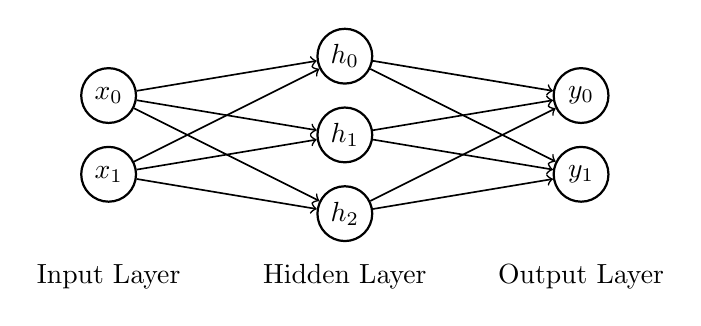
\begin{tikzpicture}
    % Input layer
    \foreach \i in {0, 1} {
      \path (0, {-\i-0.5}) coordinate [draw, circle, thick, inner sep=7pt]
            (x\i) node {$x_\i$};
    }
    \draw (0, -2.8) node {Input Layer};

    % Output layer
    \foreach \i in {0, ..., 2} {
      \path (3, {-\i}) coordinate [draw, circle, thick, inner sep=7pt]
            (h\i) node {$h_\i$};
    }
    \draw (3, -2.8) node {Hidden Layer};

    % Output layer
    \foreach \i in {0, ..., 1} {
      \path (6, {-\i-0.5}) coordinate [draw, circle, thick, inner sep=7pt]
            (y\i) node {$y_\i$};
    }
    \draw (6, -2.8) node {Output Layer};

    % Connections
      \foreach \i in {0, ..., 1} {
        \foreach \j in {0, ..., 2} {
            \draw [semithick, ->] (x\i) -- (h\j);
        }
      }
      \foreach \i in {0, ..., 2} {
        \foreach \j in {0, ..., 1} {
            \draw [semithick, ->] (h\i) -- (y\j);
        }
      }
  \end{tikzpicture}
  }
  \only<8>{
  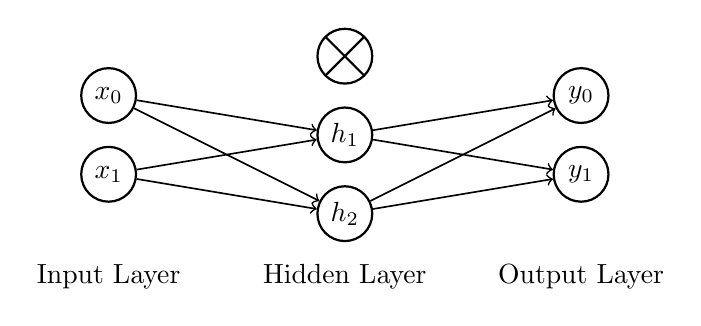
\begin{tikzpicture}[cross/.style={path picture={
  \draw[black]
(path picture bounding box.south east) -- (path picture bounding box.north west) (path picture bounding box.south west) -- (path picture bounding box.north east);
}}]
    % Input layer
    \foreach \i in {0, 1} {
      \path (0, {-\i-0.5}) coordinate [draw, circle, thick, inner sep=7pt]
            (x\i) node {$x_\i$};
    }
    \draw (0, -2.8) node {Input Layer};

    % Output layer
    \foreach \i in {1, ..., 2} {
      \path (3, {-\i}) coordinate [draw, circle, thick, inner sep=7pt] (h\i) node {$h_\i$};
    }

    % Dropped out unit
    \path (3, 0) coordinate [draw, circle, thick, inner sep=7pt, cross] (d);

    \draw (3, -2.8) node {Hidden Layer};

    % Output layer
    \foreach \i in {0, ..., 1} {
      \path (6, {-\i-0.5}) coordinate [draw, circle, thick, inner sep=7pt]
            (y\i) node {$y_\i$};
    }
    \draw (6, -2.8) node {Output Layer};

    % Connections
      \foreach \i in {0, ..., 1} {
        \foreach \j in {1, ..., 2} {
            \draw [semithick, ->] (x\i) -- (h\j);
        }
      }
      \foreach \i in {1, ..., 2} {
        \foreach \j in {0, ..., 1} {
            \draw [semithick, ->] (h\i) -- (y\j);
        }
      }
  \end{tikzpicture}
  }
  \only<9>{
  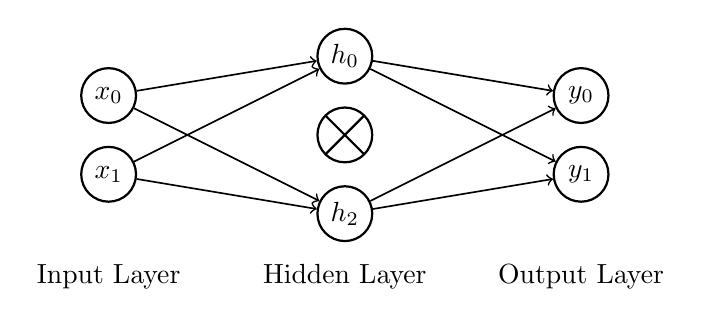
\begin{tikzpicture}[cross/.style={path picture={
  \draw[black]
(path picture bounding box.south east) -- (path picture bounding box.north west) (path picture bounding box.south west) -- (path picture bounding box.north east);
}}]
    % Input layer
    \foreach \i in {0, 1} {
      \path (0, {-\i-0.5}) coordinate [draw, circle, thick, inner sep=7pt]
            (x\i) node {$x_\i$};
    }
    \draw (0, -2.8) node {Input Layer};

    % Output layer
    \foreach \i in {0, 2} {
      \path (3, {-\i}) coordinate [draw, circle, thick, inner sep=7pt] (h\i) node {$h_\i$};
    }

    % Dropped out unit
    \path (3, -1) coordinate [draw, circle, thick, inner sep=7pt, cross] (d);

    \draw (3, -2.8) node {Hidden Layer};

    % Output layer
    \foreach \i in {0, ..., 1} {
      \path (6, {-\i-0.5}) coordinate [draw, circle, thick, inner sep=7pt]
            (y\i) node {$y_\i$};
    }
    \draw (6, -2.8) node {Output Layer};

    % Connections
      \foreach \i in {0, ..., 1} {
        \foreach \j in {0, 2} {
            \draw [semithick, ->] (x\i) -- (h\j);
        }
      }
      \foreach \i in {0, 2} {
        \foreach \j in {0, ..., 1} {
            \draw [semithick, ->] (h\i) -- (y\j);
        }
      }
  \end{tikzpicture}
  }
  \only<10>{
  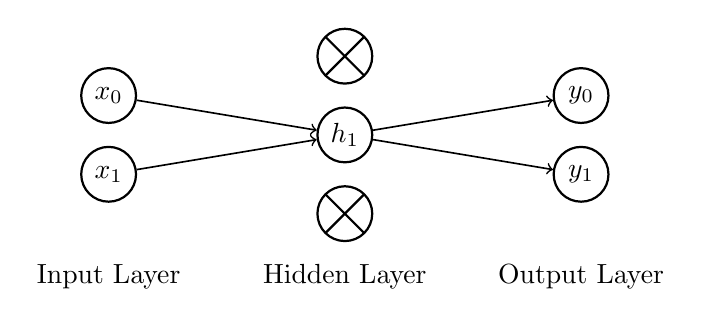
\begin{tikzpicture}[cross/.style={path picture={
  \draw[black]
(path picture bounding box.south east) -- (path picture bounding box.north west) (path picture bounding box.south west) -- (path picture bounding box.north east);
}}]
    % Input layer
    \foreach \i in {0, 1} {
      \path (0, {-\i-0.5}) coordinate [draw, circle, thick, inner sep=7pt]
            (x\i) node {$x_\i$};
    }
    \draw (0, -2.8) node {Input Layer};

    % Output layer
    \foreach \i in {1} {
      \path (3, {-\i}) coordinate [draw, circle, thick, inner sep=7pt] (h\i) node {$h_\i$};
    }

    % Dropped out unit
    \path (3, 0) coordinate [draw, circle, thick, inner sep=7pt, cross] (d1);
    \path (3, -2) coordinate [draw, circle, thick, inner sep=7pt, cross] (d2);

    \draw (3, -2.8) node {Hidden Layer};

    % Output layer
    \foreach \i in {0, ..., 1} {
      \path (6, {-\i-0.5}) coordinate [draw, circle, thick, inner sep=7pt]
            (y\i) node {$y_\i$};
    }
    \draw (6, -2.8) node {Output Layer};

    % Connections
      \foreach \i in {0, ..., 1} {
        \foreach \j in {1} {
            \draw [semithick, ->] (x\i) -- (h\j);
        }
      }
      \foreach \i in {1} {
        \foreach \j in {0, ..., 1} {
            \draw [semithick, ->] (h\i) -- (y\j);
        }
      }
  \end{tikzpicture}
  }
\end{slide}
